% Preamble
% ---
\documentclass{article}

% Packages
% ---
\usepackage{amsmath}
\usepackage{graphicx}

\begin{document}

	\title{Electronics Equations}
	\author{Tyler Hilbert}
	\date{}
	\maketitle

	\subsection*{Electronic Formula Wheel}
	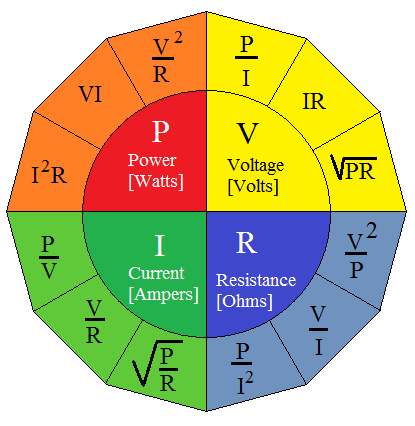
\includegraphics[width=50mm]{FormulaWheel.png}

	\subsection*{Equations from "Fundamentals of Electric Circuits"}
	% TODO - double check for all equations in chapter 1&2

	Current: $I = dQ/dt$ \smallbreak
	Note: This can also be written like this: $I = \Delta Q / \Delta t$
	%TODO - add Kirchoffs law 
	\bigskip
	
	Charge: $Q = \int_{to}^{t} i dt$
	\bigskip

	Voltage: $V = dw/dQ$ 
	\bigskip

	Power: $p = dw/dt$ 
	%TODO - check if I should add "Note that: $\sum{p} = 0$"
	\bigskip

\end{document}